\part{Teoria}

\chapter{Mobile Computing}
\label{mobile-computing}

Negli ultimi anni il numero di dispositivi connessi ad Internet è
aumentato molto velocemente, tant'è che per il 2020 ci si aspetta di
avere 50 miliardi di dispositivi connessi, per lo più mobile, anche se
per il PC resta tra gli strumenti preferiti per il mondo del lavoro.

Il termine \textbf{Mobile Computing} ha molte definizioni, che possono
essere racchiuse in ``\emph{Si parla di \textbf{Mobile Computing} quando
un processo di lavoro che prima veniva effettuato per forza in una
posizione fissa viene spostato in una posizione più dinamica}'', ovvero
racchiude tutte le tecnologie che permettono alle persone di accedere a
dei servizi \textbf{ovunque}, in qualsiasi modo e in qualsiasi momento, anche
in zone dove la connettività è limitata.

\section{Perché il mobile}

Le connessioni mobile sono molto utili in zone remote, e
anche in situazioni d'emergenza dove non c'è il tempo per costruire una rete
cablata.
Spostarsi in ambito mobile ha vari vantaggi:

\begin{itemize}
\item ci si può connettere ovunque e in ogni momento
\item con le tecnologie Wireless si possono portare le telecomunicazioni in
  ogni luogo senza bisogno di infrastruttura
\item nuove possibili applicazioni
\end{itemize}

Il mobile può essere visto sotto un punto di vista fisico, con il
device che si sposta nello spazio, o da un punto di vista logico, con il
software eseguito nel cloud.

Il bello di questo ambito è che racchiude varie branche dell'ingegneria
e pertanto viene spinto da vari fattori:

\begin{itemize}
\item \textbf{Miniaturizzazione}: device sempre più piccoli
\item \textbf{Connettività}: Wireless sempre più diffuso e performante
  (4G-LTE, Bluetooth, WiFi)
\item \textbf{Portabilità}: device più piccoli sono più facili da
  trasportare
\item \textbf{Convergenza}: lo stesso dispositivo racchiude le funzionalità
  di più dispositivi
\item \textbf{Divergenza:} creazione di dispositivi altamente specializzati
\item \textbf{App e Ecosistemi digitali}: tecnologie e applicazioni che
  interagiscono tra di loro

\end{itemize}

\section{Sfide principali}

Ci sono diverse sfide nel mondo mobile. Una di  queste è la \textbf{limitata
presenza di risorse}, dove in certi case possono essere davvero poche (si pensi
ad esempio a limitazioni di tipo energetico).

Tra le altre sfide c'è la \textbf{differenza tra il ``mondo cablato''} (per
esempio un normale computer) \textbf{e il mondo senza fili}, dove si hanno
continue disconnessioni, poca banda e ritardi variabili nelle comunicazioni.
Esistono poi problemi derivanti dai protocolli di trasferimento dati.

Anche da un punto di vista della sicurezza, \textbf{le comunicazioni senza fili
sono più facili da intercettare}, senza tener conto che i dispositivi mobili
sono passibili di furto.

\section{Ubiquitous Computing }
\label{ubiquitous-computing}

La tecnologia più avanzata è quella che tende a sparire, computer sempre
più piccoli, UI sempre più grandi (VR, AR).

Siamo quindi alla terza era del \textbf{comuputing:}

\begin{itemize}
\item[Era 1]: Mainframe computing, tanti utenti per un singolo computer
\item[Era 2]: Personal computing, un utente per ogni computer
\item[Era 3]: Ubiquitous computing, un utente per tanti computer.

\end{itemize}

\paragraph*{ParcTab} \`E stato uno dei primi dispositivi mobili. Al posto di
usare comunicazioni senza fili usava comunicazioni ad infrarossi. Grazie alla
tecnologia RFID era in grado di acquisire la sua posizione (per esempio
all'entrata di una particolare stanza un dispositivo RFID\footnote{Per
maggiori informazioni:
\url{https://it.wikipedia.org/wiki/Radio-frequency_identification}} veniva
letto, permettendo quindi di conoscere la posizione). In base al luogo in cui ci
si trovava era possibile far eseguire un'applicazione (per esempio all'interno
della stanza conferenze una \textit{shell} poteva essere automaticamente
lanciata per iniziare la presentazione). Questo fu il primo esempio di un
\textbf{device} \textit{context aware}.

\begin{figure}[H]
\minipage{0.32\textwidth}
  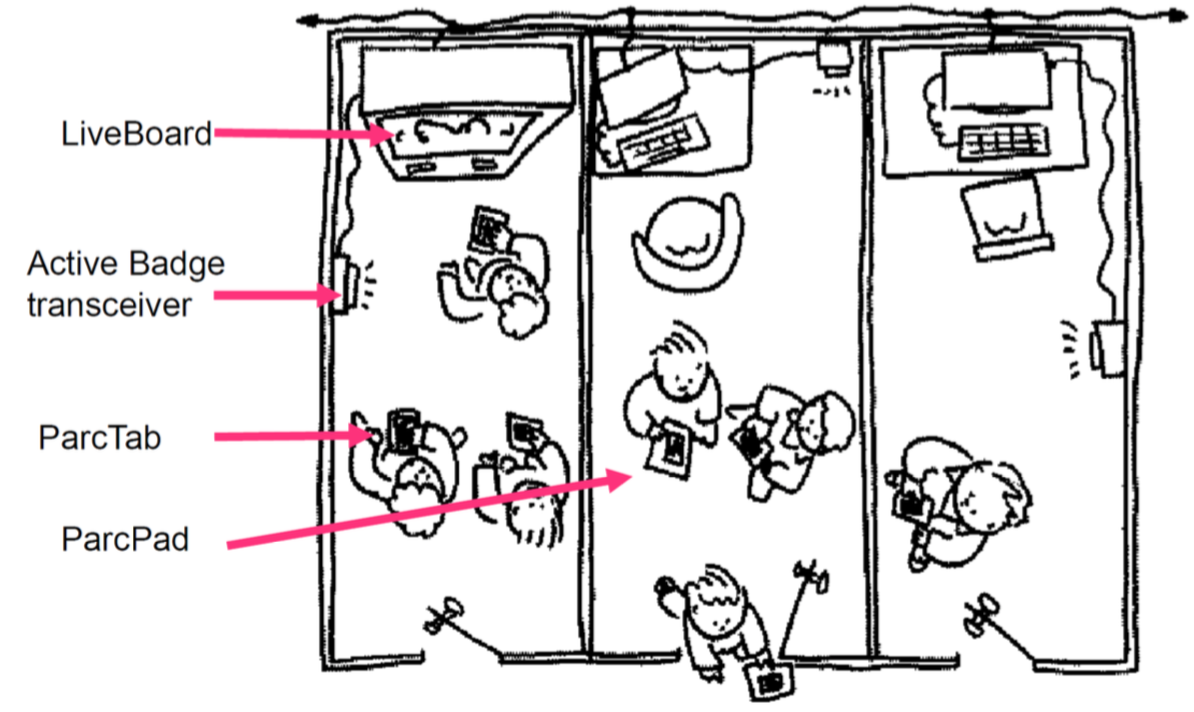
\includegraphics[scale=0.18]{image5.png}
  \caption{Funzionamento dello Xerox ParcTab}
\endminipage \hspace{75pt}
\minipage{0.32\textwidth}
  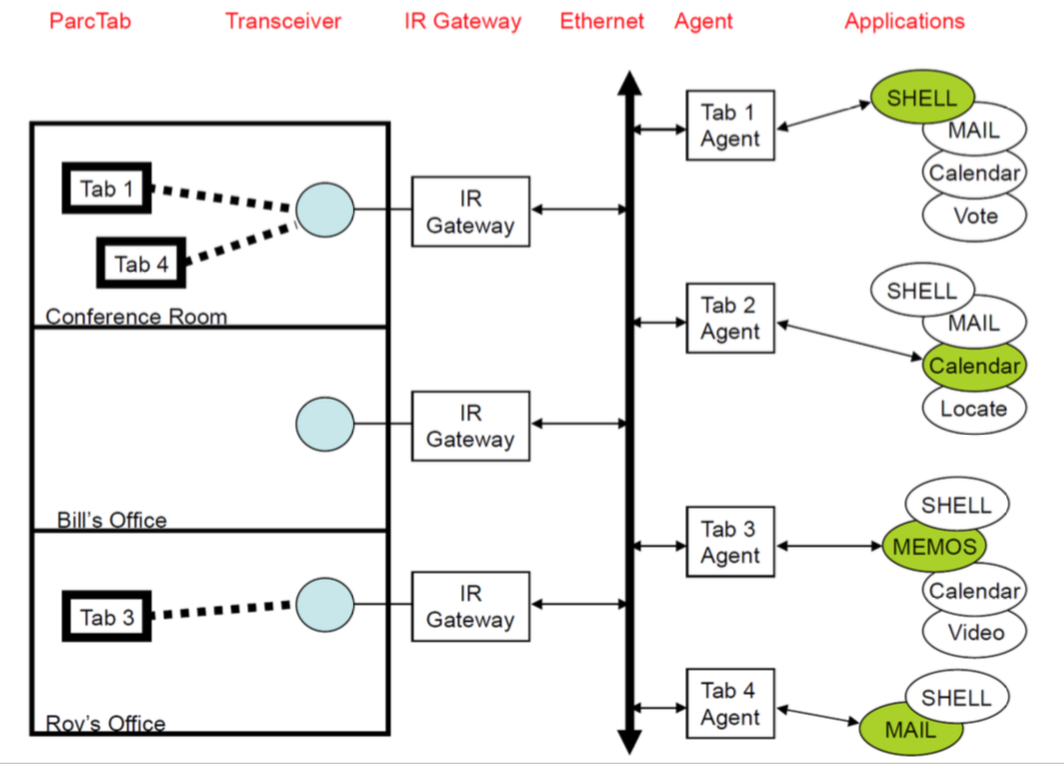
\includegraphics[scale=0.18]{image6.png}
  \caption{Esecuzioni di comnandi in base alla posizione}
\endminipage
\end{figure}

Da notare che in questa terza era non tutti i computer sono dell'utente
(smartphone, PC, ecc.) ma alcuni vengono incontrati spostandosi e
sfruttati opportunisticamente, come camere di sorveglianza, sensori,
chioschi per le informazioni, la cosa fondamentale è che tutti questi
computer siano tra loro \textbf{connessi} e \textbf{programmabili}.
Questo perché già da tempo ci sono computer in ogni dove, ma questi non
sono tra loro connessi.

Si va quindi a coprire sia i computer special purpose che quelli general
purpose, con una varietà di dispositivi enormi,

\textbf{Ubiquitous computing} è quindi una nuova era in cui le personef
sono circondate da molti computer connessi tra loro che collaborano in
modo spontaneo e che possono essere:

\begin{itemize}
\item indossati o trasportati
\item incontrati in vari luoghi
\item parte di oggetti fisici

\end{itemize}

tutti intuitivi da utilizzare e difficili da notare.
Alcune tipologie di dispositivi sono:

\begin{itemize}
\item \textbf{Sensors networks} piccoli computer dotati di sensori che
  raccolgono le informazioni sull'ambiente circostante
\item \textbf{Wearables}
\item \textbf{Networked appliances} come i distributori automatici che
  segnalano informazioni sul loro stato
\item \textbf{Smart labels} come RFID o beacon bluetooth

\end{itemize}

C'è quindi un esplosione esponenziale di dispositivi connessi ad
internet che comunicano tra loro senza che l'intervento dell'utente e
quindi la scalabilità del sistema diventi l'aspetto principale.

Ci sono quindi molte nuove sfide che derivano dalla presenza di tutti
questi dispositivi che riguardano la protezione dei dati, l'affidabilità
dei dispositivi e delle comunicazioni, la diversità e l'intrusione che
deve essere limitata per evitare di distrarre l'utente.

L'interazione con l'utente è particolarmente problematica perché deve
essere \textbf{context aware} ovvero il software deve adattarsi al
contesto in cui viene utilizzato (in macchina, in corsa, ecc) e deve
poter essere utilizzato in \textbf{varie modalità} ovvero deve
supportare più modalità di input/output in modo da potersi adattare
meglio al contesto.

\section{S.C.A.L.E.}
\label{s.c.a.l.e.}

Le sfide principali (\textbf{integrazione dei sistemi} e \textbf{humane
computing}) possono essere organizzate secondo la tassonomia SCALE:

\begin{itemize}
\item \textbf{Scalability} come supportare miliardi di dispositivi connessi
  in tutto il mondo sia a livello di connettività che di
  capacità di calcolo e integrazioni?

\item \textbf{Connectivity} come connettere tutti questi dispositivi con le
  reti wireless? Utilizzo di comunicazione ad eventi ccn il paradigma
  \textbf{push} e con la cooperazione tra i dispositivi, creando delle
  reti stratificate \textbf{P2P,} opportunistiche (ad-hoc) e allocando
  dinamicamente le risorse secondo una filosofia cloud.

\item \textbf{Adaptability} come adattare questo al contesto d'uso? Utilizzo
  dei sensori per capire il contesto, ma anche attraverso dei modelli
  predeterminati o inferendo in contesto da altre informazioni. Ma anche
  a livello utente, in base alle sue esperienze, necessità e preferenze.

\item \textbf{Liability (security)} come garantire la sicurezza? Non c'è più
  un sistema centralizzato e nella comunicazione machine-to-machine non
  è più utilizzabile il sistema di certificati, perché non si può sempre
  avere un'autorità centrale, quindi non si può fare crittografia
  end-to-end.

\item \textbf{Ease-of-use} i vari sistemi devono essere facili ed intuitivi
  da utilizzare con più modalità di input (es: movimento degli occhi,
  controlli vocali, feedback audio, ecc.)

\end{itemize}

\begin{figure}[H]
 \centering
 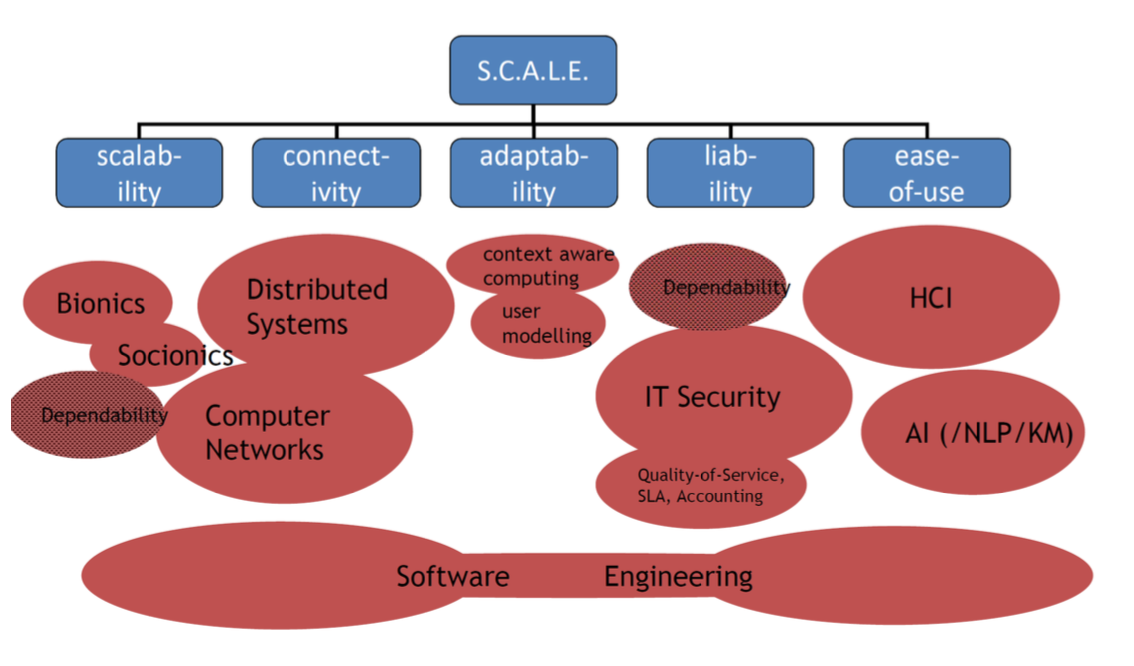
\includegraphics[scale=0.25]{image3.png}
\end{figure}

\section{Use cases/Must know}
\label{use-casesmust-know}

\paragraph*{Internet of Things} è il termine principalmente utilizzato dalla
stampa per parlare di ubiquitous computing. Ci si riferisce spesso anche con il 
termine \textit{smart devices}. I device IoT permettono agli oggetti di avere 
sensori o di essere controllati in maniera remota, attraverso strutture di rete 
già esistenti. Questo crea delle opportunità di integrazione tra il mondo 
fisico e quello dei compute, con il beneficio di una migliore efficenza, 
accuratezza e risparmio economico, in aggiunta ad un ridotto intervento umano.

\paragraph*{AutoID} standard per la definizione di etichette identificative
tramite RFID inizialmente sviluppato al MIT.

\paragraph*{OSGi} standard per la distribuzione/revisione di codice o
servizi attraverso internet per i sistemi embedded/smart. Il framework OSGi si 
propone di implementare un modello a componenti completo e dinamico cioè quello 
che manca all'ambiente Java. OSGi è organizzato in quattro \textit{layer}:
\begin{enumerate}
 \item Execution Environment (ambiente di esecuzione): è la specificazione 
dell'ambiente Java (J2SE, CDC, CLDC, MIDP, ecc.).
 \item Modules: realizza il concetto di moduli (bundle) e controlla il 
collegamento tra di loro.
 \item Life Cicle Management (Gestione del ciclo di vita): gestisce il ciclo di 
vita di un bundle senza richiedere il riavvio della VM.
 \item Service Registry: fornisce un modello di cooperazione per i bundle.
\end{enumerate}

\paragraph*{Edge Network Integration} sistema di reti ponte che
permettono di collegare reti esistenti ma basate su stack diversi.

\paragraph*{Smart home} insieme di progetti per la creazione di una casa
intelligente, inserendo attuatori e sensori nei vari oggetti per
automatizzare/risparmiare energia. Sembra più probabile
l'implementazione solo in ambito business perché ci sono investimenti
maggiori. Svolge un ruolo importante nel rendere ``intelligenti'' 
apparecchiature, impianti e sistemi.
Con \textbf{Smart home} quindi si indica un ambiente - opportunamente 
progettato e tecnologicamente attrezzato - il quale mette a disposizione 
dell'utente impianti che vanno oltre il "tradizionale", dove apparecchiature e 
sistemi sono in grado di svolgere funzioni parzialmente autonome (secondo 
reazioni a parametri ambientali di natura fissa e prestabilita) o programmate 
dall'utente o, recentemente, completamente autonome

\paragraph*{Smart item} dispositivi con risorse limitate specifici per
determinate applicazioni, ad esempio come delle smart card.

\paragraph*{LAURA} sistema di localizzazione/monitoraggio dei pazienti nelle
strutture sanitarie.

\paragraph*{DrivingStyles} progetto che studia la correlazione tra il
comportamento dell'utente nel traffico e il suo battito cardiaco. Si è infatti 
notato come uno stile di guida ``aggressivo'' porti ad avere un frequenza 
cardiaca più alta. Questo sistema riesce a capire in base allo stato 
dell'utente quanto la sua guida è pericolosa in quel momento, notificandolo in 
maniera non intrusiva. 

\paragraph*{SmartParking} occupazione e prenotazione dei parcheggi mediante
app.

\paragraph*{WaterBot} monitoraggio dei consumi di acqua in casa con aspetti
di gamification (rinforzo positivo) per incentivare il risparmio. È un modulo 
hardware che necessita di installazione e permette di dare feedback 
\textit{just-in-time} all'utente.
